% Beispiel Zitat
~\autocite[S.55]{mf2005}

% Beispiel für Bildintegration
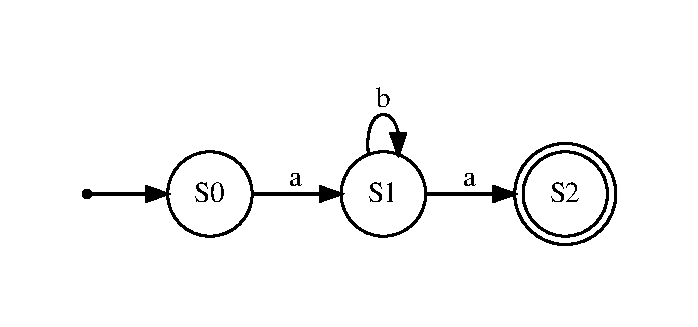
\includegraphics[width=\linewidth]{src/abbildungen/fsm}
\captionof{figure}{Bildunterschrift ~\autocite[S.14]{mf2005}}

% Beispiel für Listing
\begin{lstlisting}[language=bash,caption={Ein Listing},captionpos=b,frame=tb]
#!/bin/bash
for i in {1..10}; do
echo "$i"
done
\end{lstlisting}

% Beispiel für Tabelle
\begin{center}
\captionof{table}{Tabelle eins}
	  \begin{tabular}{ | l | c | }
	    \hline
	    Überschrift 1 & Überschrift 2 \\ \hline
	    Info 1 & Info 2 \\ \hline
	    Info 3 & Info 4 \\ \hline
	    \hline
	    \multicolumn{2}{|c|}{Info in einer Zelle} \\
	    \hline
	  \end{tabular}
\end{center}

% Beispiel für Tabelle (Booktab)
\begin{center}
  \captionof{table}{Tabelle eins}
  \begin{tabular}{ccc}\toprule
    A&B&C \\ \midrule
    a&b&c \\ \cmidrule{1-3}
    1&2&3\\ \bottomrule
  \end{tabular}
\end{center}

